\section{Introducción}

  \paragraph{}El objetivo principal del diseño arquitectónico es desarrollar una
  estructura de programa modular y representar las relaciones de control
  entre los módulos. Además el diseño arquitectónico mezcla la estructura del
  programa y la estructura de datos, definiendo además las interfaces que
  facilitan el flujo de datos a lo largo del programa.

  \paragraph{}La metodología a utilizar para representar el diseño
  arquitectónico será la técnica de los \textit{Diagramas de descomposición},
  los cuales representan aspectos del sistema que implican jerarquías, ya que
  son diagramas de estructuras que facilitan la representación jerárquica de los
  componentes del sistema o subsistema.

  \paragraph{}La notación básica de esta metodología hace uso de los componentes
  que se indican en la figura \ref{diagramaComponentes}.

  \begin{figure}[!ht]
            \begin{center}
            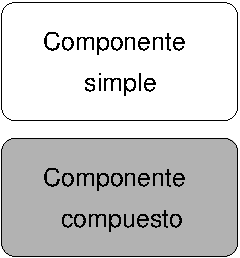
\includegraphics[]{11.Disenyo_Arquitectonico/11.1.Introduccion/Diagramas/componentes.pdf}
            \caption{Componentes de los Diagramas de descomposición.}
            \label{diagramaComponentes}
            \end{center}
         \end{figure}

  \paragraph{}El componente simple representa un componente de la arquitectura
  del sistema que no se va a refinar en más componentes. El componente
  compuesto representa un componente de la arquitectura del sistema que
  se va a descomponer en otros componentes.
